\documentclass{standalone}
\usepackage{tikz}
\usetikzlibrary{patterns, positioning}


\begin{document}
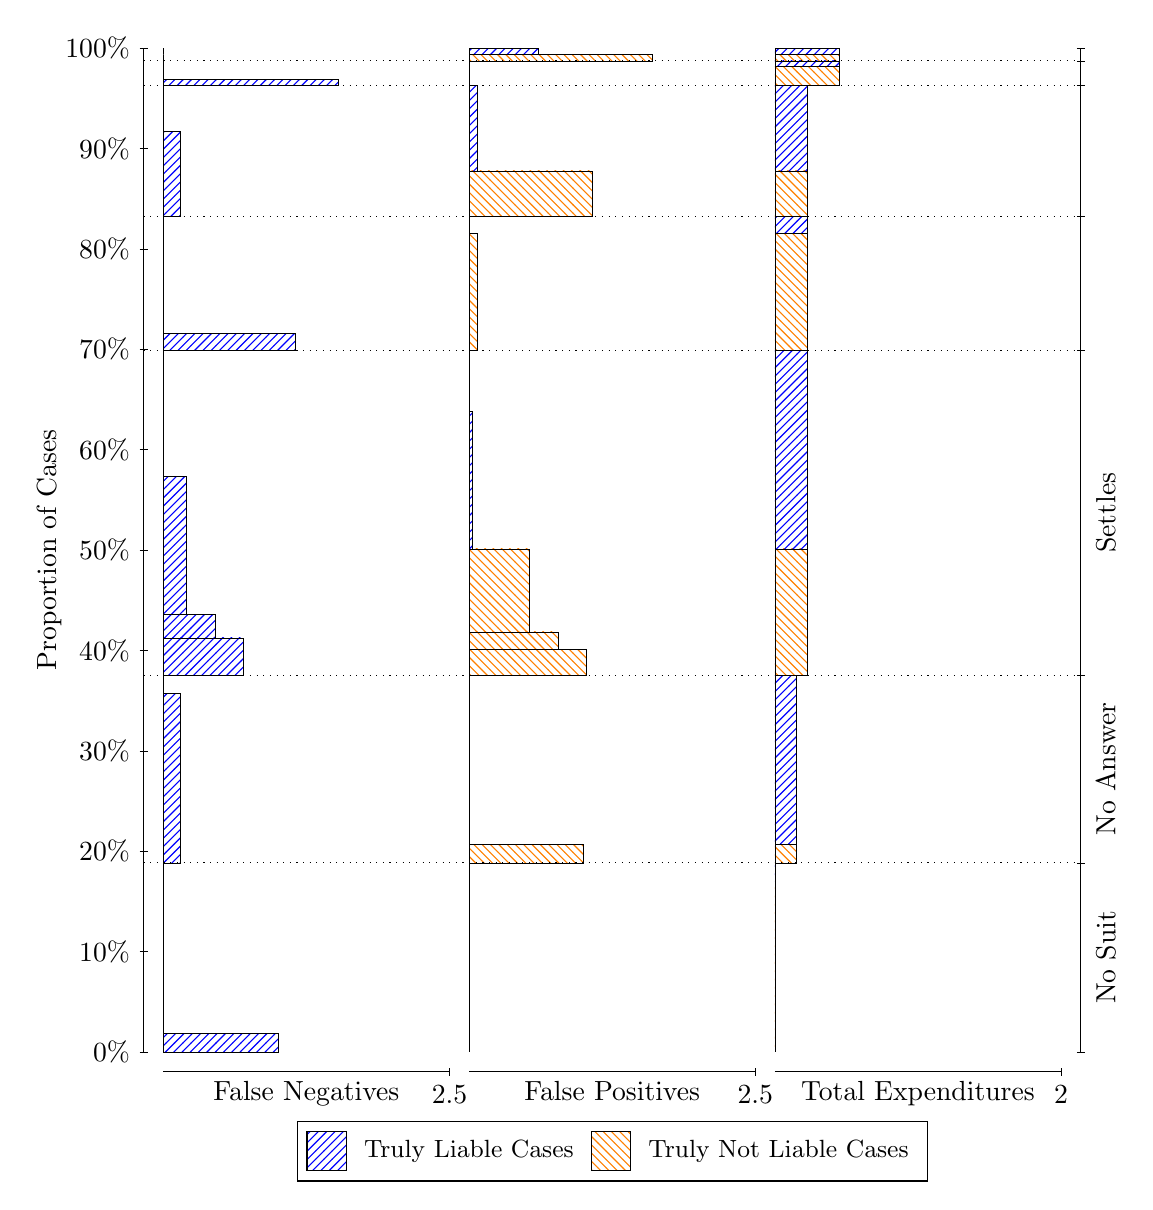
\begin{tikzpicture}
\draw[black, very thin] (1.5,1.75) -- (1.5,14.5);
\node[rotate=90, text=black, anchor=center] at (0.3, 8.125) {Proportion of Cases};
\draw[black, very thin] (1.45,1.75) -- (1.55,1.75);
\node[text=black, anchor=east] at (1.45, 1.75) {0\%};
\draw[black, very thin] (1.45,3.025) -- (1.55,3.025);
\node[text=black, anchor=east] at (1.45, 3.025) {10\%};
\draw[black, very thin] (1.45,4.3) -- (1.55,4.3);
\node[text=black, anchor=east] at (1.45, 4.3) {20\%};
\draw[black, very thin] (1.45,5.575) -- (1.55,5.575);
\node[text=black, anchor=east] at (1.45, 5.575) {30\%};
\draw[black, very thin] (1.45,6.85) -- (1.55,6.85);
\node[text=black, anchor=east] at (1.45, 6.85) {40\%};
\draw[black, very thin] (1.45,8.125) -- (1.55,8.125);
\node[text=black, anchor=east] at (1.45, 8.125) {50\%};
\draw[black, very thin] (1.45,9.4) -- (1.55,9.4);
\node[text=black, anchor=east] at (1.45, 9.4) {60\%};
\draw[black, very thin] (1.45,10.675) -- (1.55,10.675);
\node[text=black, anchor=east] at (1.45, 10.675) {70\%};
\draw[black, very thin] (1.45,11.95) -- (1.55,11.95);
\node[text=black, anchor=east] at (1.45, 11.95) {80\%};
\draw[black, very thin] (1.45,13.225) -- (1.55,13.225);
\node[text=black, anchor=east] at (1.45, 13.225) {90\%};
\draw[black, very thin] (1.45,14.5) -- (1.55,14.5);
\node[text=black, anchor=east] at (1.45, 14.5) {100\%};

\draw[black, very thin] (13.4,1.75) -- (13.4,14.5);
\draw[black, very thin] (13.35,1.75) -- (13.45,1.75);
\node[anchor=west] at (13.35, 1.75) {};
\draw[black, very thin] (13.35,4.1507) -- (13.45,4.1507);
\node[anchor=west] at (13.35, 4.1507) {};
\draw[black, very thin] (13.35,6.5342) -- (13.45,6.5342);
\node[anchor=west] at (13.35, 6.5342) {};
\draw[black, very thin] (13.35,10.66) -- (13.45,10.66);
\node[anchor=west] at (13.35, 10.66) {};
\draw[black, very thin] (13.35,12.365) -- (13.45,12.365);
\node[anchor=west] at (13.35, 12.365) {};
\draw[black, very thin] (13.35,14.021) -- (13.45,14.021);
\node[anchor=west] at (13.35, 14.021) {};
\draw[black, very thin] (13.35,14.338) -- (13.45,14.338);
\node[anchor=west] at (13.35, 14.338) {};
\draw[black, very thin] (13.35,14.5) -- (13.45,14.5);
\node[anchor=west] at (13.35, 14.5) {};

\draw[black, very thin, pattern color=blue, pattern=north east lines] (1.75,1.75) rectangle (3.2033,1.991);
\draw[black, very thin, pattern color=orange, pattern=north west lines] (1.75,1.991) rectangle (1.75,4.1507);
\draw[black, very thin, pattern color=blue, pattern=north east lines] (1.75,4.1507) rectangle (1.968,6.3017);
\draw[black, very thin, pattern color=orange, pattern=north west lines] (1.75,6.3017) rectangle (1.75,6.5342);
\draw[black, very thin, pattern color=blue, pattern=north east lines] (1.75,6.5342) rectangle (2.7673,7.0092);
\draw[black, very thin, pattern color=blue, pattern=north east lines] (1.75,7.0092) rectangle (2.404,7.3044);
\draw[black, very thin, pattern color=blue, pattern=north east lines] (1.75,7.3044) rectangle (2.0407,9.0559);
\draw[black, very thin, pattern color=orange, pattern=north west lines] (1.75,9.0559) rectangle (1.75,10.66);
\draw[black, very thin, pattern color=blue, pattern=north east lines] (1.75,10.66) rectangle (3.4213,10.88);
\draw[black, very thin, pattern color=orange, pattern=north west lines] (1.75,10.88) rectangle (1.75,12.365);
\draw[black, very thin, pattern color=blue, pattern=north east lines] (1.75,12.365) rectangle (1.968,13.445);
\draw[black, very thin, pattern color=orange, pattern=north west lines] (1.75,13.445) rectangle (1.75,14.021);
\draw[black, very thin, pattern color=blue, pattern=north east lines] (1.75,14.021) rectangle (3.9663,14.097);
\draw[black, very thin, pattern color=orange, pattern=north west lines] (1.75,14.097) rectangle (1.75,14.338);
\draw[black, very thin, pattern color=orange, pattern=north west lines] (1.75,14.338) rectangle (1.75,14.415);
\draw[black, very thin, pattern color=blue, pattern=north east lines] (1.75,14.415) rectangle (1.75,14.5);
\draw[black, very thin, pattern color=orange, pattern=north west lines] (5.6333,1.75) rectangle (5.6333,3.9097);
\draw[black, very thin, pattern color=blue, pattern=north east lines] (5.6333,3.9097) rectangle (5.6333,4.1507);
\draw[black, very thin, pattern color=orange, pattern=north west lines] (5.6333,4.1507) rectangle (7.0867,4.3832);
\draw[black, very thin, pattern color=blue, pattern=north east lines] (5.6333,4.3832) rectangle (5.6333,6.5342);
\draw[black, very thin, pattern color=orange, pattern=north west lines] (5.6333,6.5342) rectangle (7.123,6.8586);
\draw[black, very thin, pattern color=orange, pattern=north west lines] (5.6333,6.8586) rectangle (6.7597,7.0846);
\draw[black, very thin, pattern color=orange, pattern=north west lines] (5.6333,7.0846) rectangle (6.3963,8.1388);
\draw[black, very thin, pattern color=blue, pattern=north east lines] (5.6333,8.1388) rectangle (5.6697,9.8903);
\draw[black, very thin, pattern color=blue, pattern=north east lines] (5.6333,9.8903) rectangle (5.6333,10.66);
\draw[black, very thin, pattern color=orange, pattern=north west lines] (5.6333,10.66) rectangle (5.7423,12.146);
\draw[black, very thin, pattern color=blue, pattern=north east lines] (5.6333,12.146) rectangle (5.6333,12.365);
\draw[black, very thin, pattern color=orange, pattern=north west lines] (5.6333,12.365) rectangle (7.1957,12.94);
\draw[black, very thin, pattern color=blue, pattern=north east lines] (5.6333,12.94) rectangle (5.7423,14.021);
\draw[black, very thin, pattern color=orange, pattern=north west lines] (5.6333,14.021) rectangle (5.6333,14.262);
\draw[black, very thin, pattern color=blue, pattern=north east lines] (5.6333,14.262) rectangle (5.6333,14.338);
\draw[black, very thin, pattern color=orange, pattern=north west lines] (5.6333,14.338) rectangle (7.9587,14.415);
\draw[black, very thin, pattern color=blue, pattern=north east lines] (5.6333,14.415) rectangle (6.5053,14.5);
\draw[black, very thin, pattern color=orange, pattern=north west lines] (9.5167,1.75) rectangle (9.5167,3.9097);
\draw[black, very thin, pattern color=blue, pattern=north east lines] (9.5167,3.9097) rectangle (9.5167,4.1507);
\draw[black, very thin, pattern color=orange, pattern=north west lines] (9.5167,4.1507) rectangle (9.7892,4.3832);
\draw[black, very thin, pattern color=blue, pattern=north east lines] (9.5167,4.3832) rectangle (9.7892,6.5342);
\draw[black, very thin, pattern color=orange, pattern=north west lines] (9.5167,6.5342) rectangle (9.9254,8.1388);
\draw[black, very thin, pattern color=blue, pattern=north east lines] (9.5167,8.1388) rectangle (9.9254,10.66);
\draw[black, very thin, pattern color=orange, pattern=north west lines] (9.5167,10.66) rectangle (9.9254,12.146);
\draw[black, very thin, pattern color=blue, pattern=north east lines] (9.5167,12.146) rectangle (9.9254,12.365);
\draw[black, very thin, pattern color=orange, pattern=north west lines] (9.5167,12.365) rectangle (9.9254,12.94);
\draw[black, very thin, pattern color=blue, pattern=north east lines] (9.5167,12.94) rectangle (9.9254,14.021);
\draw[black, very thin, pattern color=orange, pattern=north west lines] (9.5167,14.021) rectangle (10.334,14.262);
\draw[black, very thin, pattern color=blue, pattern=north east lines] (9.5167,14.262) rectangle (10.334,14.338);
\draw[black, very thin, pattern color=orange, pattern=north west lines] (9.5167,14.338) rectangle (10.334,14.415);
\draw[black, very thin, pattern color=blue, pattern=north east lines] (9.5167,14.415) rectangle (10.334,14.5);
\draw[black, dotted] (1.5,4.1507) -- (13.4,4.1507);
\draw[black, dotted] (1.5,6.5342) -- (13.4,6.5342);
\draw[black, dotted] (1.5,10.66) -- (13.4,10.66);
\draw[black, dotted] (1.5,12.365) -- (13.4,12.365);
\draw[black, dotted] (1.5,14.021) -- (13.4,14.021);
\draw[black, dotted] (1.5,14.338) -- (13.4,14.338);
\draw[black, very thin] (1.75,1.5) -- (5.3833,1.5);
\node[text=black, anchor=north] at (3.5667, 1.5) {False Negatives};
\draw[black, very thin] (5.3833,1.45) -- (5.3833,1.55);
\node[text=black, anchor=north] at (5.3833, 1.45) {2.5};

\draw[black, very thin] (5.6333,1.5) -- (9.2667,1.5);
\node[text=black, anchor=north] at (7.45, 1.5) {False Positives};
\draw[black, very thin] (9.2667,1.45) -- (9.2667,1.55);
\node[text=black, anchor=north] at (9.2667, 1.45) {2.5};

\draw[black, very thin] (9.5167,1.5) -- (13.15,1.5);
\node[text=black, anchor=north] at (11.333, 1.5) {Total Expenditures};
\draw[black, very thin] (13.15,1.45) -- (13.15,1.55);
\node[text=black, anchor=north] at (13.15, 1.45) {2};

\node[text=black, centered, rotate=90] at (13.72, 2.9503) {No Suit};
\node[text=black, centered, rotate=90] at (13.72, 5.3425) {No Answer};
\node[text=black, centered, rotate=90] at (13.72, 8.5973) {Settles};





\draw (7.449999999999999,1.5) node[draw=none] (baseCoordinate) {};
\begin{scope}[align=center]
        \matrix[scale=0.5, draw=black, below=0.5cm of baseCoordinate, nodes={draw}, column sep=0.1cm]{
            \node[rectangle, draw, minimum width=0.5cm, minimum height=0.5cm, pattern color=blue, pattern=north east lines] {}; &
            \node[draw=none, font=\small, text=black] (B) {Truly Liable Cases}; &
            \node[rectangle, draw, minimum width=0.5cm, minimum height=0.5cm, pattern color=orange, pattern=north west lines] {}; &
            \node[draw=none, font=\small, text=black] (B) {Truly Not Liable Cases}; \\
            };
\end{scope}

\end{tikzpicture}
\end{document}